\part{Lecture 02: Markov Decision Processes}
\title[RL Lecture 02]{Lecture 02: Markov Decision Processes}
\date{}
\frame{\titlepage}

%%%%%%%%%%%%%%%%%%%%%%%%%%%%%%%%%%%%%%%%%%%%%%%%%%%%%%%%%%%%%
%% Preface / Motivation %%
%%%%%%%%%%%%%%%%%%%%%%%%%%%%%%%%%%%%%%%%%%%%%%%%%%%%%%%%%%%%%
\frame{\frametitle{Preface}
  \begin{itemize}
    \onslide<1->\item Markov decision processes (MDP) are a \hl{mathematically idealized form of RL problems}.
    \onslide<1->\item They allow precise theoretical statements (e.g., on optimal solutions).
    \onslide<1->\item They deliver insights into RL solutions since many real-world problems can be abstracted as MDPs.
    \onslide<2->\item In the following \hl{we'll focus on}:
    \onslide<2->\begin{itemize}
  \item fully observable MDPs (i.e., $\bm{x}_k=\bm{y}_k$) and
  \item finite MDPs (i.e., finite number of states \& actions).
    \end{itemize}
  \end{itemize}
  \vfill
  \onslide<3->\begin{table}
  \centering
  \begin{tabular}{M{2ex}M{2em}M{10em}M{10em}}
    %\cline{3-4}
    \multicolumn{2}{c}{\multirow{2}{*}{}}& \multicolumn{2}{c}{All states observable?}\\[1ex]
    %\cline{3-4}
    \multicolumn{2}{c}{} & Yes & No\\
    \cmidrule{3-4}
    \multirow{2}{*}{\rotatebox{90}{Actions?}} & No & Markov Chain (MC) &Hidden Markov Model (HMM)\\[2ex]
    %\cline{2-4}
    & Yes & Markov Decision Process (MDP) & Partially Observable MDP (POMDP)\\
    \cmidrule{3-4}
  \end{tabular}
  \caption{Different Markov models}
  \label{tab:DifferentMarkovModels}
  \end{table}
}

%%%%%%%%%%%%%%%%%%%%%%%%%%%%%%%%%%%%%%%%%%%%%%%%%%%%%%%%%%%%%
%% Remark: Scalar and Vectorial State/Action Representation %%
%%%%%%%%%%%%%%%%%%%%%%%%%%%%%%%%%%%%%%%%%%%%%%%%%%%%%%%%%%%%%
\frame{\frametitle{Scalar and vectorial representations in finite MDPs}
  \begin{itemize}
    \onslide<1->\item The position of a chess piece can be represented in two ways:
    \begin{itemize}
      \onslide<1->\item Vectorial: $\bm{x}=\begin{bmatrix}x_\mathrm{h} & x_\mathrm{v}\end{bmatrix}\T$, i.e., a two-element vector with horizontal and vertical information,
      \onslide<2->\item Scalar: simple enumeration of all available positions (e.g., $x=3$).
    \end{itemize}
    \onslide<3->\item Both ways represent the same amount of information.
    \onslide<3->\item \hl{We will stick to the scalar representation of states and actions in finite MDPs}.
  \end{itemize}
  \onslide<1->\begin{figure}
  \includegraphics[width=4cm]{fig/lec02/Chess_Board.pdf}
  \end{figure}
}

\frame{\frametitle{Table of contents}\tableofcontents}

%%%%%%%%%%%%%%%%%%%%%%%%%%%%%%%%%%%%%%%%%%%%%%%%%%%%%%%%%%%%%%%%%%
\section{Finite Markov chains}
%%%%%%%%%%%%%%%%%%%%%%%%%%%%%%%%%%%%%%%%%%%%%%%%%%%%%%%%%%%%%%%%%%

%%%%%%%%%%%%%%%%%%%%%%%%%%%%%%%%%%%%%%%%%%%%%%%%%%%%%%%%%%%%%
%% Markov Chain %%
%%%%%%%%%%%%%%%%%%%%%%%%%%%%%%%%%%%%%%%%%%%%%%%%%%%%%%%%%%%%%
\frame{\frametitle{Markov chain}

  \begin{defi}{Finite Markov chain}{Markov_chain}
    A \hl{finite Markov chain} is a tuple $\left\langle\mathcal{X}, \bm{\mathcal{P}} \right\rangle$ with
    \begin{itemize}
    \item $\mathcal{X}$ being a finite set of discrete-time states $X_k\in\mathcal{X}$,
    \item $\bm{\mathcal{P}}=\bm{\mathcal{P}}_{xx'}=\Pb{X_{k+1}=x'|X_{k}=x}$ is the state transition probability.
    \end{itemize}
  \end{defi}
  \pause
  \begin{itemize}
  \item Specific stochastic process model
    \pause
  \item Sequence of random variables $X_k, X_{k+1},\ldots$
    \pause
  \item `Memoryless', i.e., system properties are time invariant
    \pause
  \item In continuous-time framework: Markov Process\pause$^{\ddagger}$
  \end{itemize}
  \vfill
      {\footnotesize $^{\ddagger}$This results in a nomenclature inconsistency with Markov decision/reward `processes' in the literature.}
}

%%%%%%%%%%%%%%%%%%%%%%%%%%%%%%%%%%%%%%%%%%%%%%%%%%%%%%%%%%%%%
%% State Transistion Matrix %%
%%%%%%%%%%%%%%%%%%%%%%%%%%%%%%%%%%%%%%%%%%%%%%%%%%%%%%%%%%%%%
\frame{\frametitle{State transition matrix}

  \begin{defi}{State transition matrix}{STM}
    Given a Markov state $X_k=x$ and its successor $X_{k+1}=x'$, the \hl{state transition probability} $\forall \left\{x,x'\right\}\in \mathcal{X}$ is defined by the matrix
    \begin{equation}
      \bm{\mathcal{P}}_{xx'}=\Pb{X_{k+1}=x'|X_{k}=x} .
    \end{equation}
  \end{defi}
  \pause
  Here,  $\bm{\mathcal{P}}_{xx'}\in\Re^{n\times n}$ has the form
  \begin{equation*}
    \bm{\mathcal{P}}_{xx'} = \begin{bmatrix} p_{11} & p_{12} & \cdots & p_{1n}\\ p_{21} &  &  & \vdots\\ \vdots & & & \vdots\\ p_{n1} & \cdots & \cdots & p_{nn}\end{bmatrix}
  \end{equation*}
  with $p_{ij}\in [0,1]$ being the specific probability to go from state $x=X_i$ to state $x'=X_j$. Since this is a probability distribution, $\sum_{j} p_{ij}=1$ must hold $\forall i$.
}


%%%%%%%%%%%%%%%%%%%%%%%%%%%%%%%%%%%%%%%%%%%%%%%%%%%%%%%%%%%%%
%% Forest Markov Chain Example (1)%%
%%%%%%%%%%%%%%%%%%%%%%%%%%%%%%%%%%%%%%%%%%%%%%%%%%%%%%%%%%%%%
\frame{\frametitle{Example of a Markov chain (1)}
  \begin{minipage}[t]{0.53\linewidth}
    \vspace{0pt}
    \begin{figure}		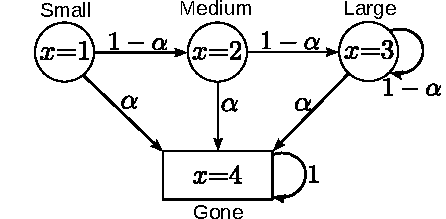
\includegraphics[width=6cm]{fig/lec02/Forest_Markov_Chain.pdf}
      \caption{Forest tree Markov chain}
      \label{fig:Forest_Markov_Chain}
    \end{figure}
  \end{minipage}
  \begin{minipage}[t]{0.45\linewidth}
    \vspace{-0.7cm}
    \begin{align*}
      x&\in\left\{1,2,3,4\right\}\\
      &=\left\{\text{small},\text{medium},\text{large},\text{gone}\right\}\\[1em]
      \bm{\mathcal{P}} &= \begin{bmatrix}0 & 1-\alpha & 0 & \alpha  \\ 0 & 0 &1-\alpha & \alpha \\ 0 & 0 &1-\alpha & \alpha \\ 0 & 0 & 0 & 1\end{bmatrix}
    \end{align*}
  \end{minipage}
  \begin{itemize}
  \item At $x=1$ a small tree is planted (`starting point').
  \item A tree grows with $(1-\alpha)$ probability.
  \item If it reaches $x=3$ (large) its growth is limited.
  \item With $\alpha$ probability a natural hazard destroys the tree.
  \item The state $x=4$ is terminal (`infinite loop').
  \end{itemize}
}

%%%%%%%%%%%%%%%%%%%%%%%%%%%%%%%%%%%%%%%%%%%%%%%%%%%%%%%%%%%%%
%% Forest Markov Chain Example (2)%%
%%%%%%%%%%%%%%%%%%%%%%%%%%%%%%%%%%%%%%%%%%%%%%%%%%%%%%%%%%%%%
\frame{\frametitle{Example of a Markov chain (2)}
  \begin{figure}
    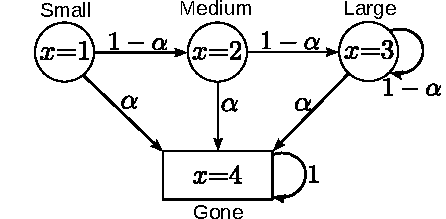
\includegraphics[height=0.5\textheight]{fig/lec02/Forest_Markov_Chain.pdf}
  \end{figure}
  Possible \hl{samples} for the given Markov chain example starting from $x=1$ (small tree):
  \begin{itemize}
  \item Small $\rightarrow$ gone
  \item Small $\rightarrow$ medium $\rightarrow$ gone
  \item Small $\rightarrow$ medium $\rightarrow$ large $\rightarrow$ gone
  \item Small $\rightarrow$ medium $\rightarrow$ large $\rightarrow$ large $\rightarrow\ldots$
  \end{itemize}
}

%%%%%%%%%%%%%%%%%%%%%%%%%%%%%%%%%%%%%%%%%%%%%%%%%%%%%%%%%%%%%%%%%%
\section{Finite Markov reward processes}
%%%%%%%%%%%%%%%%%%%%%%%%%%%%%%%%%%%%%%%%%%%%%%%%%%%%%%%%%%%%%%%%%%
\begin{frame}
  \frametitle{Table of contents}
  \tableofcontents[currentsection]
\end{frame}

%%%%%%%%%%%%%%%%%%%%%%%%%%%%%%%%%%%%%%%%%%%%%%%%%%%%%%%%%%%%%
%% Markov Reward Process %%
%%%%%%%%%%%%%%%%%%%%%%%%%%%%%%%%%%%%%%%%%%%%%%%%%%%%%%%%%%%%%
\frame{\frametitle{Markov reward process}

  \begin{defi}{Finite Markov reward process}{Markov_reward_process}
    A \hl{finite Markov reward process (MRP)} is a tuple $\left\langle\mathcal{X}, \bm{\mathcal{P}}, \hl{\mathcal{R}, \gamma} \right\rangle$ with
    \begin{itemize}
    \item $\mathcal{X}$ being a finite set of discrete-time states $X_k\in\mathcal{X}$,
    \item $\bm{\mathcal{P}}=\bm{\mathcal{P}}_{xx'}=\Pb{X_{k+1}=x'|X_{k}=x}$ is the state transition probability,
    \item \hl{$\mathcal{R}$ is a reward function, $\mathcal{R}=\mathcal{R}_x=\E{R_{k+1}|X_k=x_k}$ and}
    \item \hl{$\gamma$ is a discount factor, $\gamma\in\left\{\Re|0 \leq \gamma \leq 1\right\}$}.
    \end{itemize}
  \end{defi}
  \pause
  \begin{itemize}
  \item Markov chain extended with rewards \pause
  \item Still an autonomous stochastic process without specific inputs \pause
  \item Reward $R_{k+1}$ only depends on state $X_k$
  \end{itemize}
}

%%%%%%%%%%%%%%%%%%%%%%%%%%%%%%%%%%%%%%%%%%%%%%%%%%%%%%%%%%%%%
%% Forest Markov Reward Process %%
%%%%%%%%%%%%%%%%%%%%%%%%%%%%%%%%%%%%%%%%%%%%%%%%%%%%%%%%%%%%%
\frame{\frametitle{Example of a Markov reward process}
  \begin{figure}
    \includegraphics[height=0.5\textheight]{fig/lec02/Forest_Markov_Reward_Process.pdf}
    \caption{Forest Markov reward process}
    \label{fig:Forest_Markov_Reward_Process}
  \end{figure}

  \begin{itemize}
  \item Growing larger trees is rewarded, since it will be
    \begin{itemize}
    \item appreciated by hikers and
    \item useful for wood production.
    \end{itemize}
  \item Losing a tree due to a hazard is unrewarded.
  \end{itemize}
}

%%%%%%%%%%%%%%%%%%%%%%%%%%%%%%%%%%%%%%%%%%%%%%%%%%%%%%%%%%%%%
%% Recap Return %%
%%%%%%%%%%%%%%%%%%%%%%%%%%%%%%%%%%%%%%%%%%%%%%%%%%%%%%%%%%%%%
\frame{\frametitle{Recap on return}

  \begin{block}{Return}
    The return $G_k$ is the total discounted reward starting from step $k$ onwards. For \hl{episodic tasks} it becomes the finite series
    \begin{equation}
      G_k = R_{k+1} + \gamma R_{k+2} + \gamma^2 R_{k+3} + \cdots = \sum_{i=0}^N \gamma^i R_{k+i+1}
    \end{equation}
    terminating at step $N$ while it is an infinite series for \hl{continuing tasks}
    \begin{equation}
      G_k = R_{k+1} + \gamma R_{k+2} + \gamma^2 R_{k+3} + \cdots = \sum_{i=0}^\infty \gamma^i R_{k+i+1}\, .
    \end{equation}
  \end{block}
  \pause
  \begin{itemize}
  \item The discount $\gamma$ characterizes the decrease in present value of future rewards.
    \pause
  \item \emph{Give me a hamburger today and I will gladly repay you ... \hl{on Tuesday}.}
  \end{itemize}
}

%%%%%%%%%%%%%%%%%%%%%%%%%%%%%%%%%%%%%%%%%%%%%%%%%%%%%%%%%%%%%
%% Value in MRP %%
%%%%%%%%%%%%%%%%%%%%%%%%%%%%%%%%%%%%%%%%%%%%%%%%%%%%%%%%%%%%%
\frame{\frametitle{Value function in MRP}
  \vspace{-0.25cm}
  \begin{defi}{Value function in MRP}{value_function_MRP}
    The \hl{state-value function} $v(x_k)$ of an MRP is the expected return starting from state $x_k$
    \begin{equation}
      v(x_k) = \E{G_k \vert X_k=x_k} .
    \end{equation}
  \end{defi}
  \begin{itemize}
  \item Represents the long-term value of being in state $X_k$.
  \end{itemize}
  \vspace{0.25cm}
  \begin{figure}
    \includegraphics[height=0.325\textheight]{fig/lec02/Value_Golf.pdf}
    \caption{Isolines indicate state value of different golf ball locations (source: R. Sutton and G. Barto, Reinforcement Learning: An Introduction, 2018, \href{https://creativecommons.org/licenses/by-nc-nd/2.0/}{CC BY-NC-ND 2.0})}
    \label{fig:Value_Golf}
  \end{figure}
}

%%%%%%%%%%%%%%%%%%%%%%%%%%%%%%%%%%%%%%%%%%%%%%%%%%%%%%%%%%%%%
%% State-Value Samples Forest Markov Reward Process %%
%%%%%%%%%%%%%%%%%%%%%%%%%%%%%%%%%%%%%%%%%%%%%%%%%%%%%%%%%%%%%
\frame{\frametitle{State-value samples of forest MRP}
  \onslide<1->{\begin{figure}
      \includegraphics[height=0.5\textheight]{fig/lec02/Forest_Markov_Reward_Process.pdf}
    \end{figure}
    Exemplary \hl{samples} for $\hat{v}$ with $\gamma=0.5$ starting in $x=1$:
    \begin{alignat*}{2}
      &x=1 \rightarrow 4, &&\hat{v}= 1,\\ }
  \onslide<2->{&x=1 \rightarrow 2 \rightarrow 4, &&\hat{v}= 1 + 0.5\cdot 2=2.0,\\ }
  \onslide<3->{&x=1 \rightarrow 2 \rightarrow 3  \rightarrow 4, \quad&&\hat{v}=1+ 0.5\cdot 2+ 0.25\cdot 3=3.75,\\ }
  \onslide<4->{&x=1 \rightarrow 2 \rightarrow 3 \rightarrow 3 \rightarrow 4, \quad&&\hat{v}=1+ 0.5\cdot 2+0.25 \cdot 3+ 0.125\cdot3=4.13.}
    \end{alignat*}
}

%%%%%%%%%%%%%%%%%%%%%%%%%%%%%%%%%%%%%%%%%%%%%%%%%%%%%%%%%%%%%
%% Bellman Equation for MRPs (1)%%
%%%%%%%%%%%%%%%%%%%%%%%%%%%%%%%%%%%%%%%%%%%%%%%%%%%%%%%%%%%%%
\frame{\frametitle{Bellman equation for MRPs (1)}
  Problem: How to calculate all state values in closed form?\\
  \onslide<2->Solution: Bellman equation.
  \begin{equation}
    \onslide<3->{
      \label{eq:Bellman_MRP}
      \begin{split}
	v(x_k) &= \E{G_k \vert X_k=x_k}}\\
    &	\onslide<4->{= \E{R_{k+1} + \gamma R_{k+2} + \gamma^2 R_{k+3}+\ldots \vert X_k=x_k}}\\
    &\onslide<5->{= \E{R_{k+1} + \gamma \left(R_{k+2} + \gamma R_{k+3}+\ldots\right) \vert X_k=x_k}}\\
    &\onslide<6->{= \E{R_{k+1} + \gamma G_{k+1} \vert X_k=x_k}}\\
    &\onslide<7->{= \E{R_{k+1} + \gamma 	v(X_{k+1}) \vert X_k=x_k}}
      \end{split}
  \end{equation}
  \vspace*{\fill}
  \onslide<8->{
    \begin{figure}
      \hspace*{-1.5cm}
      \includegraphics[width=6.1cm]{fig/lec02/Back_Up_MRP.pdf}
      \caption{Backup diagram for $v(x_k)$}
      \label{fig:Back_Up_MRP}
    \end{figure}
  }
}

%%%%%%%%%%%%%%%%%%%%%%%%%%%%%%%%%%%%%%%%%%%%%%%%%%%%%%%%%%%%%
%% Bellman Equation for MRPs (2) %%
%%%%%%%%%%%%%%%%%%%%%%%%%%%%%%%%%%%%%%%%%%%%%%%%%%%%%%%%%%%%%
\frame{\frametitle{Bellman equation for MRPs (2)}
  Assuming a known reward function $\mathcal{R}(x)$ for every state $X=x\in\mathcal{X}$
  \begin{equation}
    \bm{r}_{\mathcal{X}}= \begin{bmatrix} \mathcal{R}(x_1) & \cdots & \mathcal{R}(x_n)\end{bmatrix}\T = \begin{bmatrix} \mathcal{R}_1 & \cdots & \mathcal{R}_n\end{bmatrix}\T
  \end{equation}
  for a finite number of $n$ states \pause with unknown state values
  \begin{equation}
    \bm{v}_{\mathcal{X}}= \begin{bmatrix} v(x_1) & \cdots & v(x_n)\end{bmatrix}\T = \begin{bmatrix} v_1 & \cdots & v_n\end{bmatrix}\T
  \end{equation}
  one can derive a linear equation system based on \figref{fig:Back_Up_MRP}:\pause
  \begin{equation}
    \label{eq:Bellman_MRP_linear}
    \begin{split}
      \bm{v}_{\mathcal{X}}&=\bm{r}_{\mathcal{X}}+\gamma\bm{\mathcal{P}}_{xx'}\bm{v}_{\mathcal{X}},\\
      \begin{bmatrix} v_1 \\ \vdots \\ v_n \end{bmatrix} &= \begin{bmatrix} \mathcal{R}_1 \\ \vdots \\ \mathcal{R}_n \end{bmatrix} + \gamma\begin{bmatrix} p_{11} & \cdots & p_{1n}\\ \vdots &  & \vdots\\ p_{n1} & \cdots & p_{nn}\end{bmatrix}\begin{bmatrix} v_1 \\ \vdots \\ v_n \end{bmatrix} .
    \end{split}
  \end{equation}
}

%%%%%%%%%%%%%%%%%%%%%%%%%%%%%%%%%%%%%%%%%%%%%%%%%%%%%%%%%%%%%
%% Sovling the MRP Bellman Equation %%
%%%%%%%%%%%%%%%%%%%%%%%%%%%%%%%%%%%%%%%%%%%%%%%%%%%%%%%%%%%%%
\frame{\frametitle{Solving the MRP Bellman equation}
  Above, \eqref{eq:Bellman_MRP_linear} is a normal equation in $\bm{v}_{\mathcal{X}}$:
  \begin{equation}
    \label{eq:MRP_normal_equation}
    \begin{split}
      \bm{v}_{\mathcal{X}}&=\bm{r}_{\mathcal{X}}+\gamma\bm{\mathcal{P}}_{xx'}\bm{v}_{\mathcal{X}},\\
      \Leftrightarrow \underbrace{\left(\bm{I}-\gamma\bm{\mathcal{P}}_{xx'}\right)}_{\bm{A}}\underbrace{\bm{v}_{\mathcal{X}}}_{x}&=\underbrace{\bm{r}_{\mathcal{X}}}_{\bm{b}}.
    \end{split}
  \end{equation} \pause
  Possible solutions are (among others):
  \begin{itemize}
  \item Direct inversion (Gaussian elimination, $\mathcal{O}(n^3)$),\pause
  \item Matrix decomposition (QR, Cholesky, etc. , $\mathcal{O}(n^3)$),\pause
  \item Iterative solutions (e.g., Krylov-subspaces, often better than $\mathcal{O}(n^3)$).\pause
  \end{itemize}
  \vspace{0.5cm}
  In RL identifying and solving \eqref{eq:MRP_normal_equation} is a key task, which is often realized only approximately for high-order state spaces.
}
%%%%%%%%%%%%%%%%%%%%%%%%%%%%%%%%%%%%%%%%%%%%%%%%%%%%%%%%%%%%%
%% Forest Markov Reward Process with State-Values%%
%%%%%%%%%%%%%%%%%%%%%%%%%%%%%%%%%%%%%%%%%%%%%%%%%%%%%%%%%%%%%
\frame{\frametitle{Example of a MRP with state values}
  \begin{figure}
    \includegraphics[height=0.6\textheight]{fig/lec02/Forest_Markov_Reward_Process_State_Value.pdf}
    \caption{Forest Markov reward process including state values}
    \label{fig:Forest_Markov_Chain_State_Value}
  \end{figure}
  \begin{itemize}
  \item Discount factor $\gamma=0.8$
  \item Disaster probability $\alpha=0.2$
  \end{itemize}
}

%%%%%%%%%%%%%%%%%%%%%%%%%%%%%%%%%%%%%%%%%%%%%%%%%%%%%%%%%%%%%%%%%%
\section{Finite markov decision processes}
%%%%%%%%%%%%%%%%%%%%%%%%%%%%%%%%%%%%%%%%%%%%%%%%%%%%%%%%%%%%%%%%%%
\begin{frame}
  \frametitle{Table of contents}
  \tableofcontents[currentsection]
\end{frame}

%%%%%%%%%%%%%%%%%%%%%%%%%%%%%%%%%%%%%%%%%%%%%%%%%%%%%%%%%%%%%
%% Markov Decision Process %%
%%%%%%%%%%%%%%%%%%%%%%%%%%%%%%%%%%%%%%%%%%%%%%%%%%%%%%%%%%%%%
\frame{\frametitle{Markov decision process}

  \begin{defi}{Finite Markov decision process}{Markov_decision_process}
    A \hl{finite Markov decision process (MDP)} is a tuple $\left\langle\mathcal{X}, \hl{\mathcal{U}}, \bm{\mathcal{P}}, \mathcal{R}, \gamma \right\rangle$ with
    \begin{itemize}
    \item $\mathcal{X}$ being a finite set of discrete-time states $X_k\in\mathcal{X}$,
    \item \hl{$\mathcal{U}$ as a finite set of discrete-time actions $U_k\in\mathcal{U}$,}
    \item $\bm{\mathcal{P}}=\bm{\mathcal{P}}_{xx'}^{\hl{u}}$ is the state transition probability $\bm{\mathcal{P}}=\Pb{X_{k+1}=x' \vert X_{k}=x_k, \hl{U_{k}=u_k}}$,
    \item $\mathcal{R}$ is a reward function, $\mathcal{R}=\mathcal{R}_x^{\hl{u}}=\E{R_{k+1} \vert X_k=x_k, \hl{U_{k}=u_k}}$ and
    \item $\gamma$ is a discount factor, $\gamma\in\left\{\Re \vert 0 \leq \gamma \leq 1\right\}$.
    \end{itemize}
  \end{defi}
  \pause
  \begin{itemize}
  \item Markov reward process is extended with actions / decisions.
  \item Now, rewards also depend on action $U_k$.
  \end{itemize}
}

%%%%%%%%%%%%%%%%%%%%%%%%%%%%%%%%%%%%%%%%%%%%%%%%%%%%%%%%%%%%%
%% Forest Markov Decision Process (1) %%
%%%%%%%%%%%%%%%%%%%%%%%%%%%%%%%%%%%%%%%%%%%%%%%%%%%%%%%%%%%%%
\frame{\frametitle{Example of a Markov decision process (1)}
  \begin{figure}
    \includegraphics[height=0.5\textheight]{fig/lec02/Forest_Markov_Decision_Process.pdf}
    \caption{Forest Markov decision process}
    \label{fig:Forest_Markov_Decision_Process}
  \end{figure}
  \begin{itemize}
  \item Two actions possible in each state:
    \begin{itemize}
    \item Wait $u=w$: let the tree grow.
    \item Cut $u=c$: gather the wood.
    \end{itemize}
  \item With increasing tree size the wood reward increases as well.
  \end{itemize}
}

%%%%%%%%%%%%%%%%%%%%%%%%%%%%%%%%%%%%%%%%%%%%%%%%%%%%%%%%%%%%%
%% Forest Markov Decision Process (2) %%
%%%%%%%%%%%%%%%%%%%%%%%%%%%%%%%%%%%%%%%%%%%%%%%%%%%%%%%%%%%%%
\frame{\frametitle{Example of a Markov decision process (2)}
  For the previous example the state transition probability matrix and reward function are:
  \begin{align*}
    \bm{\mathcal{P}}_{xx'}^{u=c} &=
    \begin{bmatrix}
      0 & 0 & 0 & 1  \\ 0 & 0 &0 & 1 \\ 0 & 0 &0 & 1 \\ 0 & 0 & 0 & 1
    \end{bmatrix}
    &
    \bm{\mathcal{P}}_{xx'}^{u=w} &=
    \begin{bmatrix}
      0 & 1-\alpha & 0 & \alpha  \\ 0 & 0 &1-\alpha & \alpha \\ 0 & 0 &1-\alpha & \alpha \\ 0 & 0 & 0 & 1
    \end{bmatrix}
    \\[2ex]
    \bm{r}_{\mathcal{X}}^{u=c} &= \begin{bmatrix}1 & 2 & 3 & 0 \end{bmatrix}\T
    &
    \bm{r}_{\mathcal{X}}^{u=w} &= \begin{bmatrix}0 & 0 & 1 & 0 \end{bmatrix}\T
  \end{align*}
  \begin{itemize}
  \item The term $\bm{r}_{\mathcal{X}}^u$ is the abbreviated form for receiving the output of $\mathcal{R}$ for the entire state space $\mathcal{X}$ given the action $u$.
  \end{itemize}
}

%%%%%%%%%%%%%%%%%%%%%%%%%%%%%%%%%%%%%%%%%%%%%%%%%%%%%%%%%%%%%
%% Policy (1) %%
%%%%%%%%%%%%%%%%%%%%%%%%%%%%%%%%%%%%%%%%%%%%%%%%%%%%%%%%%%%%%
\frame{\frametitle{Policy (1)}
  \vspace{-0.2cm}
  \onslide<1->{
    \begin{defi}{Policy in MDP (1)}{Policy_MDP}
      In an MDP environment, a \hl{policy} is a distribution over actions given states:
      \begin{equation}
        \label{eq:Policy_MDP}
	\pi(u_k \vert x_k)=\Pb{U_k=u_k   \vert  X_k=x_k}\, .
      \end{equation}
    \end{defi}
  }
  \vspace{-0.05cm}
  \begin{itemize}
    \onslide<2->{\item In MDPs, policies depend only on the current state.}
    \onslide<3->{\item A policy fully defines the agent's behavior (which might be stochastic or deterministic).}
  \end{itemize}
  \onslide<1->{
    \begin{figure}
      \includegraphics[height=0.35\textheight]{fig/lec02/monopoly.jpg}
      \caption{What is your best Monopoly policy? (source: Ylanite Koppens on \href{https://www.pexels.com/de-de/foto/begrifflich-brettspiel-drinnen-farben-776654/}{Pexels})}
    \end{figure}
  }
}

%%%%%%%%%%%%%%%%%%%%%%%%%%%%%%%%%%%%%%%%%%%%%%%%%%%%%%%%%%%%%
%% Policy (2) %%
%%%%%%%%%%%%%%%%%%%%%%%%%%%%%%%%%%%%%%%%%%%%%%%%%%%%%%%%%%%%%
\frame{\frametitle{Policy (2)}
  Given a finite MDP $\left\langle\mathcal{X}, \mathcal{U}, \bm{\mathcal{P}}, \mathcal{R}, \gamma \right\rangle$ and a policy $\bm{\pi}$:
  \begin{itemize}
  \item The state sequence $X_k, X_{k+1},\ldots$ is a Markov chain $\left\langle\mathcal{X}, \bm{\mathcal{P}}^{\pi} \right\rangle$ since the state transition probability depends only on the current state:
    \begin{equation}
      \bm{\mathcal{P}}_{xx'}^{\pi}=\sum_{u_k\in\mathcal{U}}\bm{\pi}(u_k \vert x_k)\bm{\mathcal{P}}_{xx'}^{u}\, .
    \end{equation}\pause
  \item Consequently, the sequence $X_k, R_{k+1}, X_{k+1},R_{k+2},\ldots$ of states and rewards is a Markov reward process $\left\langle\mathcal{X}, \bm{\mathcal{P}}^{\pi}, \mathcal{R}^{\pi}, \gamma \right\rangle$:
    \begin{equation}
      \mathcal{R}_{xx'}^{\pi}=\sum_{u_k\in\mathcal{U}}\bm{\pi}(u_k \vert x_k)\mathcal{R}_{x}^{u}\, .
    \end{equation}
  \end{itemize}
}

%%%%%%%%%%%%%%%%%%%%%%%%%%%%%%%%%%%%%%%%%%%%%%%%%%%%%%%%%%%%%
%% Recap on Value functions %%
%%%%%%%%%%%%%%%%%%%%%%%%%%%%%%%%%%%%%%%%%%%%%%%%%%%%%%%%%%%%%
\frame{\frametitle{Recap on MDP value functions}

  \begin{defi}{State-value function}{state_value_MDP}
    The state-value function of an MDP is the expected return starting in $x_k$ following policy $\pi$:
    \begin{equation*}
      v_\pi(x_k) = \El{G_k \vert X_k=x_k}{\pi}=\El{\left. \sum_{i=0}^\infty \gamma^i R_{k+i+1}\right\vert X_k}{\pi}\,.
    \end{equation*}
  \end{defi}
  \pause
  \begin{defi}{Action-value function}{action_value_MDP}
    The action-value function of an MDP is the expected return starting in $x_k$ taking action $u_k$ following policy $\pi$:
    \begin{equation*}
      q_\pi(x_k,u_k) = \El{G_k \vert X_k=x_k, U_k=u_k}{\pi}=\El{\left.\sum_{i=0}^\infty \gamma^i R_{k+i+1}\right\vert X_k, U_k}{\pi}\, .
    \end{equation*}
  \end{defi}
}

%%%%%%%%%%%%%%%%%%%%%%%%%%%%%%%%%%%%%%%%%%%%%%%%%%%%%%%%%%%%%
%% Bellman Expectation Equation (1) %%
%%%%%%%%%%%%%%%%%%%%%%%%%%%%%%%%%%%%%%%%%%%%%%%%%%%%%%%%%%%%%
\frame{\frametitle{Bellman expectation equation (1)}
  Similarly to \eqref{eq:Bellman_MRP}, an MDP state value can be decomposed using a Bellman equation:
  \begin{equation}
    v_\pi(x_k)	= \El{R_{k+1} + \gamma 	v_{\pi}(X_{k+1}) \vert X_k=x_k}{\pi}\, .
  \end{equation}
  \pause
  In finite MDPs, the state value can be directly linked to the action value (cf.~\figref{fig:Back_Up_Value_MDP}):
  \begin{equation}
    \label{eq:v_MDP_finite}
    v_\pi(x_k)	= \sum_{u_k\in\mathcal{U}}\pi(u_k \vert x_k)q_\pi(x_k,u_k) \, .
  \end{equation}
  \pause
  \vspace{0.5cm}
  \begin{figure}
    \hspace*{-1.5cm}
    \includegraphics[width=6.5cm]{fig/lec02/Back_Up_Value_MDP.pdf}
    \caption{Backup diagram for $v_{\pi}(x_k)$}
    \label{fig:Back_Up_Value_MDP}
  \end{figure}
}

%%%%%%%%%%%%%%%%%%%%%%%%%%%%%%%%%%%%%%%%%%%%%%%%%%%%%%%%%%%%%
%% Bellman Expectation Equation (2) %%
%%%%%%%%%%%%%%%%%%%%%%%%%%%%%%%%%%%%%%%%%%%%%%%%%%%%%%%%%%%%%
\frame{\frametitle{Bellman expectation equation (2)}
  Likewise, the action value of an MDP can be decomposed into a Bellman notation:
  \begin{equation}
    q_\pi(x_k,u_k)	= \El{R_{k+1} + \gamma 	q_{\pi}(X_{k+1},U_{k+1}) \vert X_{k}=x_{k},U_{k}=u_{k}}{\pi}\, .
  \end{equation}
  \pause
  In finite MDPs, the action value can be directly linked to the state value (cf.~\figref{fig:Back_Up_Action_Value_MDP}):
  \begin{equation}
    \label{eq:q_MDP_finite}
    q_\pi(x_k,u_k)	= \mathcal{R}^u_x + \gamma \sum_{x_{k+1}\in\mathcal{X}}p_{xx'}^u v_\pi(x_{k+1}) \, .
  \end{equation}
  \pause
  \vspace{0.5cm}
  \begin{figure}
    \hspace*{-1.5cm}
    \includegraphics[width=6.5cm]{fig/lec02/Back_Up_Action_Value_MDP.pdf}
    \caption{Backup diagram for $q_{\pi}(x_k,u_k)$}
    \label{fig:Back_Up_Action_Value_MDP}
  \end{figure}
}

%%%%%%%%%%%%%%%%%%%%%%%%%%%%%%%%%%%%%%%%%%%%%%%%%%%%%%%%%%%%%
%% Bellman Expectation Equation (3) %%
%%%%%%%%%%%%%%%%%%%%%%%%%%%%%%%%%%%%%%%%%%%%%%%%%%%%%%%%%%%%%
\frame{\frametitle{Bellman expectation equation (3)}
  Inserting \eqref{eq:q_MDP_finite} into \eqref{eq:v_MDP_finite} directly results in:
  \begin{equation}
    \label{eq:Bellman_MDP_linear_non_matrix}
    v_\pi(x_k)	= \sum_{u_k\in\mathcal{U}}\pi(u_k \vert x_k)\left(\mathcal{R}^u_x + \gamma\sum_{x_{k+1}\in\mathcal{X}}p_{xx'}^u v_\pi(x_{k+1})\right) \, .
  \end{equation}
  \pause
  Conversely, the action value becomes:
  \begin{equation}
    q_\pi(x_k,u_k)	= \mathcal{R}^u_x + \gamma\sum_{x_{k+1}\in\mathcal{X}}p_{xx'}^u \left(\sum_{u_{k+1}\in\mathcal{U}}\pi(u_{k+1} \vert x_{k+1})q_\pi(x_{k+1},u_{k+1})\right) \, .
  \end{equation}
}

%%%%%%%%%%%%%%%%%%%%%%%%%%%%%%%%%%%%%%%%%%%%%%%%%%%%%%%%%%%%%
%% Bellman Expectation Equation in Matrix Form %%
%%%%%%%%%%%%%%%%%%%%%%%%%%%%%%%%%%%%%%%%%%%%%%%%%%%%%%%%%%%%%
\frame{\frametitle{Bellman expectation equation in matrix form}
  Given a policy $\pi$ and following the same assumptions as for \eqref{eq:Bellman_MRP_linear}, the Bellman expectation equation can be expressed in matrix form:
  \begin{equation}
    \label{eq:Bellman_MDP_linear}
    \begin{split}
      \bm{v}_{\mathcal{X}}^{\pi}&=\bm{r}_{\mathcal{X}}^{\pi}+\gamma\bm{\mathcal{P}}_{xx'}^{\pi}\bm{v}_{\mathcal{X}}^{\pi},\\
      \begin{bmatrix} v_{1}^{\pi} \\ \vdots \\ v_{n}^{\pi} \end{bmatrix} &= \begin{bmatrix} \mathcal{R}_{1}^{\pi} \\ \vdots \\ \mathcal{R}_{n}^{\pi} \end{bmatrix} + \gamma\begin{bmatrix} p_{11}^{\pi} & \cdots & p_{1n}^{\pi}\\ \vdots &  & \vdots\\ p_{n1}^{\pi} & \cdots & p_{nn}^{\pi}\end{bmatrix}\begin{bmatrix} v_{1}^{\pi} \\ \vdots \\ v_{n}^{\pi} \end{bmatrix}.
    \end{split}
  \end{equation}
  Here, $\bm{r}_{\mathcal{X}}^{\pi}$ and $\bm{\mathcal{P}}_{xx'}^{\pi}$ are the rewards and state transition probability following policy $\pi$. \pause Hence, the state value can be calculated by solving \eqref{eq:Bellman_MDP_linear} for $\bm{v}_{\mathcal{X}}^{\pi}$, e.g., by direct matrix inversion:
  \begin{equation}
    \bm{v}_{\mathcal{X}}^{\pi}=\left(\bm{I}-\gamma\bm{\mathcal{P}}_{xx'}^{\pi}\right)^{-1}\bm{r}_{\mathcal{X}}^{\pi}.
  \end{equation}
}

%%%%%%%%%%%%%%%%%%%%%%%%%%%%%%%%%%%%%%%%%%%%%%%%%%%%%%%%%%%%%
%% Bellman Expectation Equation Applied to Forest Tree Example (1)%%
%%%%%%%%%%%%%%%%%%%%%%%%%%%%%%%%%%%%%%%%%%%%%%%%%%%%%%%%%%%%%
\frame{\frametitle{Bellman expectation equation \& forest tree example (1)}
  Assume system is following a very simple policy (`\textit{fifty-fifty}')
  \begin{equation*}
    \pi(u = \text{cut} \vert x) = 0.5, \quad \pi(u = \text{wait} \vert x) = 0.5 \quad\forall x\in\mathcal{X} \, .
  \end{equation*}
  \pause
  Applied to the given environment behavior
  \begin{alignat*}{2}
    \bm{\mathcal{P}}_{xx'}^{u=c} &= \begin{bmatrix}0 & 0 & 0 & 1  \\ 0 & 0 &0 & 1 \\ 0 & 0 &0 & 1 \\ 0 & 0 & 0 & 1\end{bmatrix}, \quad \bm{\mathcal{P}}_{xx'}^{u=w} &&= \begin{bmatrix}0 & 1-\alpha & 0 & \alpha  \\ 0 & 0 &1-\alpha & \alpha \\ 0 & 0 &1-\alpha & \alpha \\ 0 & 0 & 0 & 1\end{bmatrix},\\
	\bm{r}_{\mathcal{X}}^{u=c} &= \begin{bmatrix}1 & 2 & 3 & 0 \end{bmatrix}\T, \quad \bm{r}_{\mathcal{X}}^{u=w} &&= \begin{bmatrix}0 & 0 & 1 & 0 \end{bmatrix}\T ,
  \end{alignat*}
  \pause
  one receives:
  \begin{equation*}
    \bm{\mathcal{P}}_{xx'}^{\pi} = \begin{bmatrix}0 & \frac{1-\alpha}{2} & 0 & \frac{1+\alpha}{2}  \\ 0 & 0 &\frac{1-\alpha}{2} & \frac{1+\alpha}{2} \\ 0 & 0 &\frac{1-\alpha}{2} & \frac{1+\alpha}{2} \\ 0 & 0 & 0 & 1\end{bmatrix}, \quad\bm{r}_{\mathcal{X}}^{\pi} = \begin{bmatrix}0.5 \\ 1 \\ 2 \\ 0 \end{bmatrix} .
  \end{equation*}
}

%%%%%%%%%%%%%%%%%%%%%%%%%%%%%%%%%%%%%%%%%%%%%%%%%%%%%%%%%%%%%
%% Bellman Expectation Equation Applied to Forest Tree Example (2)%%
%%%%%%%%%%%%%%%%%%%%%%%%%%%%%%%%%%%%%%%%%%%%%%%%%%%%%%%%%%%%%
\frame{\frametitle{Bellman expectation equation \& forest tree example (2)}
  \begin{figure}
    %\hspace*{-1.5cm}
    \includegraphics[height=0.6\textheight]{fig/lec02/Forest_Markov_Decision_Process_State_Value.pdf}
    \caption{Forest MDP with fifty-fifty policy including state values}
    \label{fig:Forest_Markov_Decision_Process_State_Value}
  \end{figure}
  \begin{itemize}
  \item Discount factor $\gamma=0.8$
  \item Disaster probability $\alpha=0.2$
  \end{itemize}
}

%%%%%%%%%%%%%%%%%%%%%%%%%%%%%%%%%%%%%%%%%%%%%%%%%%%%%%%%%%%%%
%% Bellman Expectation Equation Applied to Forest Tree Example (3)%%
%%%%%%%%%%%%%%%%%%%%%%%%%%%%%%%%%%%%%%%%%%%%%%%%%%%%%%%%%%%%%
\frame{\frametitle{Bellman expectation equation \& forest tree example (3)}
  Using the Bellman expectation eq. \eqref{eq:q_MDP_finite} the action values can be directly calculated:
  \vspace{0.5cm}
  \begin{figure}
    \hspace*{0.5cm}
    \includegraphics[height=0.6\textheight]{fig/lec02/Forest_Markov_Decision_Process_Action_Value.pdf}
    \caption{Forest MDP with fifty-fifty policy plus action values}
    \label{fig:Forest_Markov_Decision_Process_Action_Value}
  \end{figure}
}

%%%%%%%%%%%%%%%%%%%%%%%%%%%%%%%%%%%%%%%%%%%%%%%%%%%%%%%%%%%%%%%%%%
\section{Optimal policies and value functions}
%%%%%%%%%%%%%%%%%%%%%%%%%%%%%%%%%%%%%%%%%%%%%%%%%%%%%%%%%%%%%%%%%%
\begin{frame}
  \frametitle{Table of contents}
  \tableofcontents[currentsection]
\end{frame}

%%%%%%%%%%%%%%%%%%%%%%%%%%%%%%%%%%%%%%%%%%%%%%%%%%%%%%%%%%%%%
%% Optimal Value Functions in MDP %%
%%%%%%%%%%%%%%%%%%%%%%%%%%%%%%%%%%%%%%%%%%%%%%%%%%%%%%%%%%%%%
\frame{\frametitle{Optimal value functions in an MDP}
  \begin{defi}{Optimal state-value function}{optimal_state_value_MDP}
    The optimal state-value function of an MDP is the maximum state-value function over all polices:
    \begin{equation}
      v^*(x) = \max_{\pi} v_{\pi}(x)\,.
    \end{equation}
  \end{defi}
  \vspace{-0.2cm}
  \pause
  \begin{defi}{Optimal action-value function}{optimal_action_value_MDP}
    The optimal action-value function of an MDP is the maximum action-value function over all polices:
    \begin{equation}
      q^*(x,u) = \max_{\pi} q_\pi(x,u)\, .
    \end{equation}
  \end{defi}
  \vspace{-0.1cm}
  \pause
  \begin{itemize}
  \item The optimal value function denotes the best possible agent's performance for a given MDP / environment. \pause
  \item \hl{A (finite) MDP can be easily solved in an optimal way if $q^*(x,u)$ is known.}
  \end{itemize}
}

%%%%%%%%%%%%%%%%%%%%%%%%%%%%%%%%%%%%%%%%%%%%%%%%%%%%%%%%%%%%%
%% Optimal Policy in MDP %%
%%%%%%%%%%%%%%%%%%%%%%%%%%%%%%%%%%%%%%%%%%%%%%%%%%%%%%%%%%%%%
\frame{\frametitle{Optimal policy in an MDP}
  Define a partial ordering over polices
  \begin{equation}
    \pi \geq \pi' \quad \text{if} \quad v_{\pi}(x) \geq v_{\pi'}(x) \quad \forall x\in\mathcal{X} \,.
  \end{equation}
  \pause
  \begin{theo}{Optimal policies in MDPs}{Optimal_policies_MDP}
    For any finite MDP
    \begin{itemize}
    \item there exists an optimal policy $\pi^*\geq\pi$ that is better or equal to all other policies,
    \item all optimal policies achieve the same optimal state-value function $v^*(x)=v_{\pi^*}(x)$,
    \item all optimal policies achieve the same optimal action-value function $q^*(x, u)=q_{\pi^*}(x, u)$.
    \end{itemize}
  \end{theo}
}

%%%%%%%%%%%%%%%%%%%%%%%%%%%%%%%%%%%%%%%%%%%%%%%%%%%%%%%%%%%%%
%% Bellman Optimality Equation (1)%%
%%%%%%%%%%%%%%%%%%%%%%%%%%%%%%%%%%%%%%%%%%%%%%%%%%%%%%%%%%%%%
\frame{\frametitle{Bellman optimality equation (1)}
  \onslide<1->{
    \begin{theo}{Bellman's principle of optimality}{bellman_principle_optimality}
      ``\textit{An optimal policy has the property that whatever the initial state and initial decision are, the remaining decisions must constitute an optimal policy with regard to the state resulting from the first decision.}''(R.E. Bellman, Dynamic Programming, 1957)
    \end{theo}
  }
  \begin{itemize}
    \onslide<2->{\item Any policy (i.e., also the optimal one) must satisfy the self-consistency condition given by the Bellman expectation equation.}
    \onslide<3->{\item An optimal policy must deliver the maximum expected return being in a given state:}
  \end{itemize}
  \onslide<4->{
    \begin{equation}
      \begin{split}
	v^*(x_k) &= \max_{u} q_{\pi^*}(x_k, u)\, ,}\\
  &\onslide<5->{= \max_{u} \El{G_k \vert X_k=x_k, U=u}{\pi^*}\, ,}\\
  &\onslide<6->{= \max_{u} \El{R_{k+1} + \gamma G_{k+1} \vert X_k=x_k, U=u}{\pi^*}\, ,}\\
  &\onslide<7->{= \max_{u} \E{R_{k+1} + \gamma v^*(X_{k+1}) \vert X_k=x_k, U=u}\, .}
      \end{split}
    \end{equation}
}

%%%%%%%%%%%%%%%%%%%%%%%%%%%%%%%%%%%%%%%%%%%%%%%%%%%%%%%%%%%%%
%% Bellman Optimality Equation (2)%%
%%%%%%%%%%%%%%%%%%%%%%%%%%%%%%%%%%%%%%%%%%%%%%%%%%%%%%%%%%%%%
\frame{\frametitle{Bellman optimality equation (2)}
  Again, the Bellman optimality equation can be visualized by a backup diagram:
  \begin{figure}
    %\hspace*{-1.5cm}
    \includegraphics[width=4.5cm]{fig/lec02/Back_Up_Value_Optimal_MDP.pdf}
    \caption{Backup diagram for $v^*(x_k)$}
    \label{fig:Back_Up_Value_Optimal_MDP}
  \end{figure}
  \pause
  For a finite MDP, the following expression results:
  \begin{equation}
    \label{eq:Bellman_Optimal_State_Value_MDP}
    v^*(x_k) = \max_{u_k}\, \mathcal{R}^u_x+ \gamma \sum_{x_{k+1}\in\mathcal{X}}p_{xx'}^u v_{\pi^*}(x_{k+1}) .
  \end{equation}
}

%%%%%%%%%%%%%%%%%%%%%%%%%%%%%%%%%%%%%%%%%%%%%%%%%%%%%%%%%%%%%
%% Bellman Optimality Equation (3)%%
%%%%%%%%%%%%%%%%%%%%%%%%%%%%%%%%%%%%%%%%%%%%%%%%%%%%%%%%%%%%%
\frame{\frametitle{Bellman optimality equation (3)}
  Likewise, the Bellman optimality equation is applicable to the action value:
  \begin{equation}
    q^*(x_k,u_k) = \E{R_{k+1}+ \gamma \max_{u_{k+1}} q^*(X_{k+1},U_{k+1}) \vert X_k=x_k, U_k=u_k} .
  \end{equation}
  \pause
  And, in the finite MDP case:
  \begin{equation}
    \label{eq:Bellman_Optimal_action_Value_MDP}
    q^*(x_k,u_k) = \mathcal{R}^u_x + \gamma \sum_{x_{k+1}\in\mathcal{X}}p_{xx'}^u \max_{u_{k+1}}q^*(x_{k+1}, u_{k+1}) .
  \end{equation}
  \pause
  \begin{figure}
    %\hspace*{-1.5cm}
    \includegraphics[width=4.7cm]{fig/lec02/Back_Up_Action_Value_Optimal_MDP.pdf}
    \caption{Backup diagram for $q^*(x_k,u_k)$}
    \label{fig:Back_Up_Action_Value_Optimal_MDP}
  \end{figure}
}

%%%%%%%%%%%%%%%%%%%%%%%%%%%%%%%%%%%%%%%%%%%%%%%%%%%%%%%%%%%%%
%% Solving the Bellman Optimality Equation %%
%%%%%%%%%%%%%%%%%%%%%%%%%%%%%%%%%%%%%%%%%%%%%%%%%%%%%%%%%%%%%
\frame{\frametitle{Solving the Bellman optimality equation}
  \begin{itemize}
  \item In finite MDPs with $n$ states, \eqref{eq:Bellman_Optimal_State_Value_MDP} delivers an \hl{algebraic equation system} with $n$ unknowns and $n$ \hl{state-value equations}. \pause
  \item Likewise, \eqref{eq:Bellman_Optimal_action_Value_MDP} delivers an algebraic equation system with up to $n\cdot m$ unknowns and $n \cdot m$ \hl{action-value equations} ($m=$number of actions). \pause
  \end{itemize}
  \vspace{0.5cm}
  \begin{itemize}
  \item If environment is exactly known, solving for $v^*$ or $q^*$ directly delivers optimal policy.
    \begin{itemize}
    \item If $v(x)$ is known, a one-step-ahead search is required to get $q(x, u)$.
    \item If $q(x, u)$ is known, directly choose $q^*$. \pause
    \end{itemize}
  \item Even though above decisions are very short sighted (one-step-ahead search for $v$ or direct choice of $q$), by Bellman's principle of optimality one receives the long-term maximum of the expected reward.
  \end{itemize}
}

%%%%%%%%%%%%%%%%%%%%%%%%%%%%%%%%%%%%%%%%%%%%%%%%%%%%%%%%%%%%%
%% Optimal Forest MDP %%
%%%%%%%%%%%%%%%%%%%%%%%%%%%%%%%%%%%%%%%%%%%%%%%%%%%%%%%%%%%%%
\frame{\frametitle{Optimal policy for forest tree MDP}
  Remember the forest tree MDP example:
  \begin{figure}
    \includegraphics[height=0.5\textheight]{fig/lec02/Forest_Markov_Decision_Process_No_Color.pdf}
    \label{fig:Forest_Markov_Decision_Process_No_Color}
  \end{figure}

  \begin{itemize}
  \item Two actions possible in each state:
    \begin{itemize}
    \item Wait $u=w$: let the tree grow.
    \item Cut $u=c$: gather the wood.
    \end{itemize}
  \item Lets first calculate $v^*(x)$ and then $q^*(x,u)$.
  \end{itemize}
}

%%%%%%%%%%%%%%%%%%%%%%%%%%%%%%%%%%%%%%%%%%%%%%%%%%%%%%%%%%%%%
%% Optimal Policy for Forest Tree MDP: State-Value (1)%%
%%%%%%%%%%%%%%%%%%%%%%%%%%%%%%%%%%%%%%%%%%%%%%%%%%%%%%%%%%%%%
\frame{\frametitle{Optimal policy for forest tree MDP: state value (1)}
  \vspace{-0.15cm}
  \onslide<1->{Start with $v(x=4)$ (`gone') and then continue going backwards:}
  \onslide<2->{
    \begin{align*}
      v^*(x=4) &= 0\, ,}\\
  \onslide<3->{v^*(x=3) &= \max \begin{cases} 1 + \gamma\left[(1-\alpha)v^*(x=3) + \alpha v^*(x=4)\right]\, ,\\ 3+\gamma v^*(x=4)\, ,\end{cases}}\\
  &\onslide<4->{= \max \begin{cases} 1 + \gamma\left[(1-\alpha)v^*(x=3)\right]\, ,\\ 3\, ,\end{cases}}\\\
  \onslide<5->{v^*(x=2) &= \max \begin{cases} 0 + \gamma\left[(1-\alpha)v^*(x=3) + \alpha v^*(x=4)\right]\, ,\\ 2+\gamma v^*(x=4)\, ,\end{cases}}\\
  &\onslide<6->{= \max \begin{cases} \gamma\left[(1-\alpha)v^*(x=3)\right]\, ,\\ 2\, ,\end{cases}}\\
  \onslide<7->{v^*(x=1) &= \max \begin{cases} \gamma\left[(1-\alpha)v^*(x=2)\right]\, ,\\ 1\, .\end{cases}}
    \end{align*}
}

%%%%%%%%%%%%%%%%%%%%%%%%%%%%%%%%%%%%%%%%%%%%%%%%%%%%%%%%%%%%%
%% Optimal Policy for Forest Tree MDP: State-Value (2)%%
%%%%%%%%%%%%%%%%%%%%%%%%%%%%%%%%%%%%%%%%%%%%%%%%%%%%%%%%%%%%%
\frame{\frametitle{Optimal policy for forest tree MDP: state value (2)}
  \begin{itemize}
  \item Possible solutions:
    \begin{itemize}
    \item numerical optimization approach (e.g., simplex method, gradient descent,...)
    \item manual case-by-case equation solving (dynamic programming, cf. next lecture)
    \end{itemize}
  \end{itemize}
  \begin{figure}
    \includegraphics[height=0.6\textheight]{fig/lec02/Forest_Markov_Decision_Process_Optimal_State_Value.pdf}
    \caption{State values under optimal policy ($\gamma=0.8$,	$\alpha=0.2$)}
    \label{fig:Forest_Markov_Decision_Process_Optimal_State_Value}
  \end{figure}
}

%%%%%%%%%%%%%%%%%%%%%%%%%%%%%%%%%%%%%%%%%%%%%%%%%%%%%%%%%%%%%
%% Optimal Policy for Forest Tree MDP: State-Value (3)%%
%%%%%%%%%%%%%%%%%%%%%%%%%%%%%%%%%%%%%%%%%%%%%%%%%%%%%%%%%%%%%
\frame{\frametitle{Optimal policy for forest tree MDP: state value (3)}
  \begin{figure}
    \includegraphics[height=0.6\textheight]{fig/lec02/Forest_Markov_Decision_Process_Optimal_State_Value_Gamma09.pdf}
    \caption{State values under optimal policy (\hl{$\gamma=0.9$},	$\alpha=0.2$)}
    \label{fig:Forest_Markov_Decision_Process_Optimal_State_Value_Gamma09}
  \end{figure}
}

%%%%%%%%%%%%%%%%%%%%%%%%%%%%%%%%%%%%%%%%%%%%%%%%%%%%%%%%%%%%%
%% Optimal Policy for Forest Tree MDP: Action-Value (1)%%
%%%%%%%%%%%%%%%%%%%%%%%%%%%%%%%%%%%%%%%%%%%%%%%%%%%%%%%%%%%%%
\frame{\frametitle{Optimal policy for forest tree MDP: action value (1)}
  \onslide<1->{Use $u_{k+1}=u'$ to set up equation system:
    \begin{align*}
      q^*(x=1,u=c) &= 1\, ,}\\
  \onslide<2->{q^*(x=1,u=w) &= \gamma(1-\alpha)\max_{u'}q^*(x=2,u')\, ,}\\
  \onslide<3->{q^*(x=2,u=c) &= 2\, ,}\\
  \onslide<4->{q^*(x=2,u=w) &= \gamma(1-\alpha)\max_{u'}q^*(x=3,u')\, ,}\\
  \onslide<5->{q^*(x=3,u=c) &= 3\, ,}\\
  \onslide<6->{q^*(x=3,u=w) &= 1+\gamma(1-\alpha)\max_{u'}q^*(x=3,u')\, .}
    \end{align*}
    \onslide<7->{
      \begin{itemize}
      \item There are six action-state pairs in total.
      \item Three of them can be directly determined.
      \item Three unknowns and three equations remain.
      \end{itemize}
    }
}

%%%%%%%%%%%%%%%%%%%%%%%%%%%%%%%%%%%%%%%%%%%%%%%%%%%%%%%%%%%%%
%% Optimal Policy for Forest Tree MDP: Action-Value (2)%%
%%%%%%%%%%%%%%%%%%%%%%%%%%%%%%%%%%%%%%%%%%%%%%%%%%%%%%%%%%%%%
\frame{\frametitle{Optimal policy for forest tree MDP: action value (2)}
  \onslide<1->{
    Rearrange $\max$ expressions for unknown action values:
    \begin{align*}
      q^*(x=1,u=w) &= \gamma(1-\alpha)\max\begin{cases}\gamma(1-\alpha)\max\begin{cases}1+\gamma(1-\alpha)q^*(3,w),\\3,\end{cases}\\2,\end{cases}}\\
  \onslide<2->{q^*(x=2,u=w) &= \gamma(1-\alpha)\max\begin{cases}1+\gamma(1-\alpha)q^*(3,w),\\3,\end{cases}}\\
  \onslide<3->{q^*(x=3,u=w) &= 1+\gamma(1-\alpha)\max\begin{cases}q^*(3,w),\\3.\end{cases}\,}
    \end{align*}
    \onslide<4->{Again, retrieve unknown optimal action values by numerical optimization solvers or manual backwards calculation (dynamic programming).}
}

%%%%%%%%%%%%%%%%%%%%%%%%%%%%%%%%%%%%%%%%%%%%%%%%%%%%%%%%%%%%%
%% Optimal Policy for Forest Tree MDP: Action-Value (3)%%
%%%%%%%%%%%%%%%%%%%%%%%%%%%%%%%%%%%%%%%%%%%%%%%%%%%%%%%%%%%%%
\frame{\frametitle{Optimal policy for forest tree MDP: action value (3)}
  \begin{figure}
    \includegraphics[height=0.6\textheight]{fig/lec02/Forest_Markov_Decision_Process_Optimal_Action_Value.pdf}
    \caption{Action values under optimal policy ($\gamma=0.8$,	$\alpha=0.2$)}
    \label{fig:Forest_Markov_Decision_Process_Optimal_Action_Value}
  \end{figure}
}

%%%%%%%%%%%%%%%%%%%%%%%%%%%%%%%%%%%%%%%%%%%%%%%%%%%%%%%%%%%%%
%% Optimal Policy for Forest Tree MDP: Action-Value (4)%%
%%%%%%%%%%%%%%%%%%%%%%%%%%%%%%%%%%%%%%%%%%%%%%%%%%%%%%%%%%%%%
\frame{\frametitle{Optimal policy for forest tree MDP: action value (4)}
  \begin{figure}
    \includegraphics[height=0.6\textheight]{fig/lec02/Forest_Markov_Decision_Process_Optimal_Action_Value_Gamma09.pdf}
    \caption{Action values under optimal policy (\hl{$\gamma=0.9$},	$\alpha=0.2$)}
    \label{fig:Forest_Markov_Decision_Process_Optimal_Action_Value_Gamma09}
  \end{figure}
}

%%%%%%%%%%%%%%%%%%%%%%%%%%%%%%%%%%%%%%%%%%%%%%%%%%%%%%%%%%%%%
%% Solving an MDP by Calculating Optimal State and Action-Values%%
%%%%%%%%%%%%%%%%%%%%%%%%%%%%%%%%%%%%%%%%%%%%%%%%%%%%%%%%%%%%%
\frame{\frametitle{Direct numerical state and action-value calculation}
  \begin{itemize}
  \item Possible only for \hl{small action and state-space} MDPs
    \begin{itemize}
    \item `Solving' Backgammon with $\approx 10^{20}$ states?
    \end{itemize}
    \pause
  \item Another issue: total \hl{environment knowledge} required
  \end{itemize}
  \pause
  \begin{block}{Framing the reinforcement learning problem}
    Facing the above issues, RL addresses mainly two topics:
    \begin{itemize}
    \item Approximate solutions of complex decision problems.
    \item Learning of such approximations based on data retrieved from environment interactions potentially without any a priori model knowledge.
    \end{itemize}

  \end{block}
}

%%%%%%%%%%%%%%%%%%%%%%%%%%%%%%%%%%%%%%%%%%%%%%%%%%%%%%%%%%%%%
%% Summary %%
%%%%%%%%%%%%%%%%%%%%%%%%%%%%%%%%%%%%%%%%%%%%%%%%%%%%%%%%%%%%%
\begin{frame}
  \frametitle{Summary: what you've learned in this lecture}
  \begin{itemize}
  \item Differentiate finite Markov process models with or w/o rewards and actions.\pause
  \item Interpret such stochastic processes as simplified abstractions of real-world problems.\pause
  \item Understand the importance of value functions to describe the agent's performance. \pause
  \item Formulate value-function equation systems by the Bellman principle.\pause
  \item Recognize optimal policies.\pause
  \item Setting up nonlinear equation systems for retrieving optimal policies by the Bellman principle.\pause
  \item Solving for different value functions in MRP/MDP by brute force optimization.
  \end{itemize}
\end{frame}
